\documentclass[lang=cn,a4paper,newtx,bibend=bibtex]{elegantpaper}
\usepackage{env}
\title{Problems of Chapter 9}
\author{张志心 \ 计科2106}
\date{\zhdate{2024/03/25}}
\usepackage{env}
\pgfplotsset{compat=1.17}
\addbibresource[location=local]{reference.bib}
\begin{document}
\maketitle

\begin{prob}[Exercise 9.5]
  \textbf{Theorem 9.4.} \quad The relative error of an approximate
   solution is bounded by ites relative residual.
  \[
    \dfrac{1}{\cond (A)} \dfrac{\| \rB\|_2}{\| \bB\|_2}
    \le \dfrac{\| \eB \|_2}{\| \xB \|_2}
    \le \cond (A) \dfrac{\| \rB\|_2}{\| \bB\|_2}
  \]
\end{prob}

\begin{proof}
  根据矩阵范数的定义,$\| A\|_2 = \sup\left\{\dfrac{\| A\xB\|_2}{\|\xB\|_2} : \xB \in \RBB^n, \xB \neq 0\right \}$,
  因为 $A \eB = \rB, A^{-1}\bB = \xB$,所以
  \[
    \| A\|_2\| \eB \|_2 \ge \| A\eB \|_2 \ge \| \rB \|_2, 
    \quad
    \| A^{-1} \|_2 \| \bB \|_2 \ge \| A^{-1}\bB \|_2 \ge \| \xB \|_2,
  \]

  又因为 $\cond (A) = \| A\|_2 \| A^{-1}\|_2$,所以,
  \begin{equation*}
  \begin{aligned} 
    &\| A\|_2 \|A^{-2}\|_2 \|\eB\|_2\|\bB\|_2 \ge \|\rB\|_2\|\xB\|_2 \\
    \Rightarrow \quad &\cond (A) \|\eB\|_2\|\bB\|_2 \ge \|\rB\|_2\|\xB\|_2 \\
    \Rightarrow \quad &\dfrac{1}{\cond(A)} \dfrac{\|\rB\|_2}{\|\bB\|_2} \le 
                                     \dfrac{\|\eB\|_2}{\|\xB\|_2}
  \end{aligned}
  \end{equation*}
  另一边类似,因为 $A\xB = \bB, A^{-1}\rB = \eB$,所以,
  \[
    \| A\|_2\| \xB \|_2 \ge \| A\xB \|_2 \ge \| \bB \|_2, 
    \quad
    \| A^{-1} \|_2 \| \rB \|_2 \ge \| A^{-1}\rB \|_2 \ge \| \eB \|_2,
  \]
  所以,
  \begin{equation*}
    \begin{aligned} 
      &\| A\|_2 \|A^{-2}\|_2 \|\xB\|_2\|\rB\|_2 \ge \|\bB\|_2\|\eB\|_2 \\
      \Rightarrow \quad &\cond (A) \|\xB\|_2\|\rB\|_2 \ge \|\bB\|_2\|\eB\|_2 \\
      \Rightarrow \quad &\dfrac{\|\eB\|_2}{\|\xB\|_2} \le \cond (A) 
                         \dfrac{\|\rB\|_2}{\|\bB\|_2}
    \end{aligned}
    \end{equation*}
\end{proof}

\begin{prob}[Exercise 9.8]
  What are the values of $\cond(A)$, for $A$ in (7.13) for $n = 8$ and $n = 1024$?
  \[
    A = \dfrac1{h^2}
    \begin{bmatrix}
      2 & - 1 & & & & \\
      -1 & 2 & -1 & & & \\
      & -1 & 2 & -2 & & \\
      & & \ddots & \ddots & \ddots & \\
      & & & -1 & 2 & -1 \\
      & & & & -1 & 2
    \end{bmatrix}
  \]
\end{prob}

\begin{solution}
  根据 Lemma 7.25,
  \[
    \lambda_k (A) = \dfrac{4}{h^2} \sin^2 \dfrac{k\pi}{2n}, k = 1, 2, \cdots, n - 1
  \]
  因为 $A^T = A$,所以
  \[
    \|A\|_2 = \sqrt{\rho(A^T A)} = \rho (A) = \dfrac{4}{h^2} \sin \dfrac{(n - 1)\pi}{2n}
    = \dfrac{4}{h^2} \cos \dfrac{\pi}{2n},
  \]
  因为 $\lambda^k(A^{-1}) = \lambda_k(A)^{-1}$,所以 $\|A^{-1}\|_2 = \dfrac{1}{\dfrac{4}{h^2} \sin^2 \dfrac{\pi}{2n}}$。
  所以
  \[
    \cond(A) = \| A\|_2 \|A^{-1}\|_2 = \dfrac{\cos^2 \frac{\pi}{2n}}{\sin^2 \frac{\pi}{2n}} = \cot^2 \dfrac{\pi}{2n},
  \]
  当 $n = 8$ 时,$\cond(A) \approx 25.2741$;
  当 $n = 1024$ 时,$\cond(A) \approx 424971.2 $。

\end{solution}

\begin{prob}[Exercise 9.11]
  For $\Omega = (0, 1)$, plot to show that the maximum
   wavenumber that is representable
  on $\Omega^h$ is $n_{\max} = \frac1h$.
  What if we require that the Fourier mode be $0$ at 
  the boundary points? 
\end{prob}

\begin{solution}
  为了在离散网格 $\Omega^h$ 上表示更多的波数,
  结果如图(a)所示,取 $n = 10, h = \frac{1}{n}$。
  \begin{figure}[H]
    \centering
    \begin{subfigure}[b]{0.38\textwidth}
        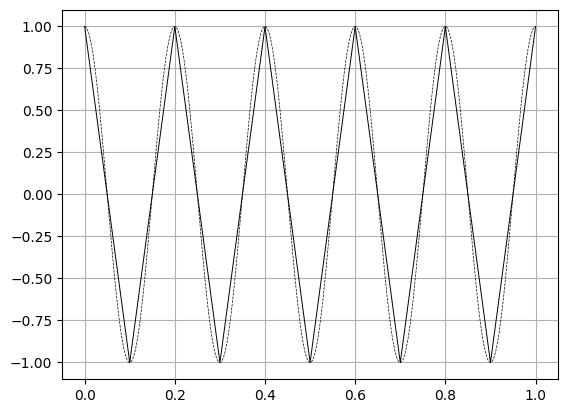
\includegraphics[width=\textwidth]{p1.png}
        \caption{$n = 10, k = 10$}
    \end{subfigure}
    \begin{subfigure}[b]{0.38\textwidth}
        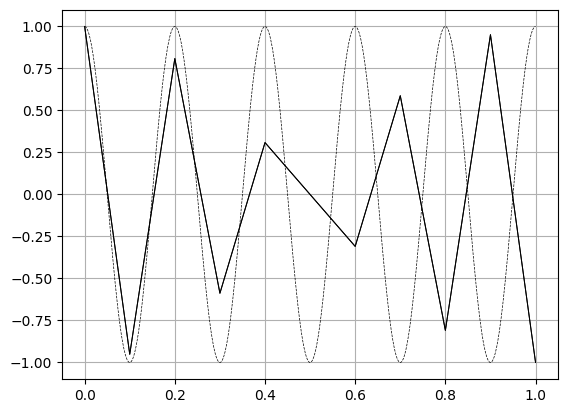
\includegraphics[width=\textwidth]{p2.png}
        \caption{$n = 10, k \in \{9,11\}$}
    \end{subfigure}
    \\
    \begin{subfigure}[b]{0.38\textwidth}
      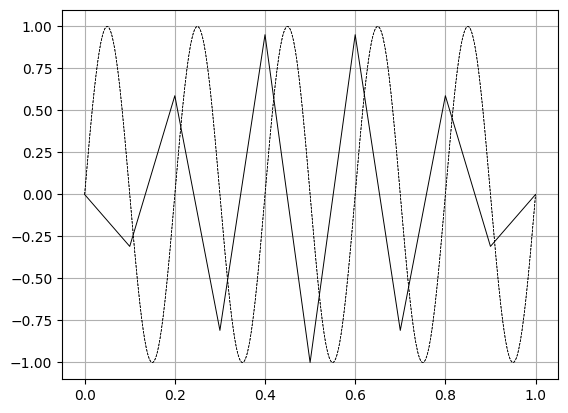
\includegraphics[width=\textwidth]{p3.png}
      \caption{$n = 10, k = 11$}
  \end{subfigure}
  \begin{subfigure}[b]{0.38\textwidth}
      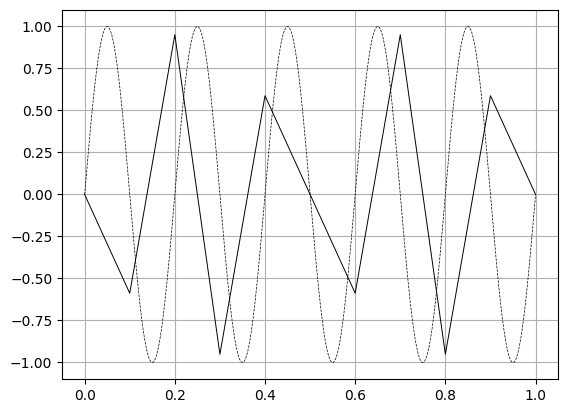
\includegraphics[width=\textwidth]{p4.png}
      \caption{$n = 10, k = 12$}
  \end{subfigure}
  \caption{Exercise 9.11}
  \end{figure}
  若取 $k = 11$ 得到的结果与 $k = 9$ 相同,都只能展示 $n - 1$ 个半波,如图(b)所示。
  因此可以得到结论,$n_{\max} = \frac{1}{h}$。

  若设置边界位置为0,
  因为 $\sin(n\pi x_i) \equiv 0, x_i = \frac{i}{n}, i = 0, \dots, n$,
  此时最多展示 $n - 1$ 个半波,如图(c)所示,若取 $k = n + 2$,
  则可以展示 $n - 2$ 个半波,如图(d)所示。
\end{solution}

\begin{prob}[Exercise 9.14]
  Plot the case of $n = 6$ for Example 9.13.
\end{prob}

\begin{solution}
  绘制 $\sin \frac32 n \pi x$ 和 $-\sin\frac12 n \pi x$ 的图像,
  以及在 $n = 6$ 的离散网格处的点值,
  可以发现在网格处两个函数重合。
  两个函数在此网格上都只能描述出 3 个半波。

  \begin{figure}[H]
    \centering
    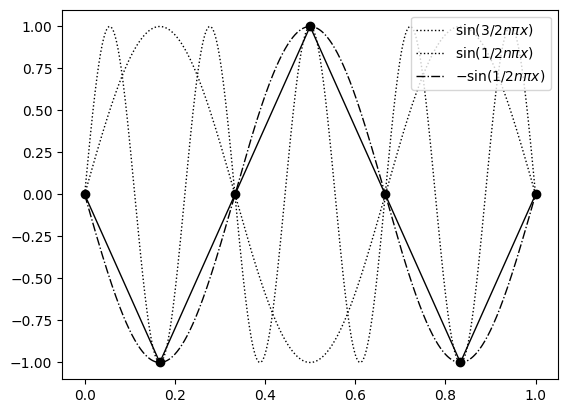
\includegraphics[width=0.5\textwidth]{p5.png}
    \caption{Example 9.13}
  \end{figure}
\end{solution}

\begin{prob}[Exercise 9.17]
  \textbf{Lemma 9.16} \quad For the linear system (9.7), the
  weighted Jacobi in Definition 8.9 has the iteration matrix
\[
  T_{\omega} = (1 - \omega)I + \omega D^{-1} (L + U) = I - \dfrac{\omega h^2}2 A,
\]
whose eigenvectors are the same as those of $A$, with the corresponding eigenvalues as
\[
  \lambda_k (T_{\omega}) = 1 - 2\omega \sin^2 \dfrac{k\pi}{2n},
\]
where $k = 1, 2, \ldots, n - 1$.
\end{prob}

\begin{proof}
  根据 Definition 8.9,方程 $\boxed{A\xB = \bB}$ 的带权 Jacobi 迭代为
  \[
    \xB^{(k + 1)} = (1 - \omega) \xB^{(k)} + \omega [T_J \xB^{(k)} + c]
  \]
  其中 $T_J = D^{-1} (L + U)$,$D, -L, -U$ 分别表示 $A$ 的对角、下三角,上三角部分。
  所以,
  \begin{equation*}\begin{aligned}
  T_{\omega} &= (1 - \omega)I + \omega D^{-1} (L + U) \\
  &= (1 - \omega)I + \omega \left(\frac2{h^2} I\right)^{-1} (-A + D) \\
  &= (1 - \omega)I + \frac{\omega h^2}{2} \left(-A + \left(\frac2{h^2} I\right)\right) \\
  &= (1 - \omega)I - \frac{\omega h^2}{2} A + \omega I\\
  &= I - \frac{\omega h^2}{2} A.
  \end{aligned}\end{equation*}

  $A$ 的特征值为 $\lambda_k(A) = \frac4{h^2} \sin^2 \frac{k\pi}{2n}$,
  设对应的特征向量为 $v_k$,$k= 1,2,\dots, n-1$。
  \begin{equation*}
    \begin{aligned}
    T_{\omega} v_k &= \left(1 - \frac{\omega h^2}{2}A\right) v_k 
      = v_k - \frac{\omega h^2}{2} A v_k \\
      &= v_k - \frac{\omega h^2}{2}\lambda_k v_k 
      = \left(1 - \frac{\omega h^2}{2} \lambda_k\right) v_k\\
      &= \left(1 - 2\omega \sin^2 \frac{k\pi}{2n}\right) v_k
      \Rightarrow \lambda_k(T_{\omega}) = 1 - 2\omega \sin^2 \frac{k\pi}{2n}
    \end{aligned}
  \end{equation*}

  
\end{proof}

\begin{prob}[Exercise 9.18]
  Write a program to reproduce Fig. 2.7 in
  the book by Briggs et al. [2000]. For $n = 64$, $\omega \in [0, 1]$,
  verify $\rho (T_{\omega}) \ge 0.9986$ and hence slow convergence.
\end{prob}

\begin{solution}
  当 $n = 64, \omega \in (0, 1)$ 时,
  根据图上的单调性,可以得知
  \[
    \rho(T_{\omega}) = \lambda_{\max} > 1 - 2 \sin^2\frac{\pi}{2n} \approx 0.9988
  \]
  所以收敛速度很缓慢。
\begin{figure}[H]
  \centering
  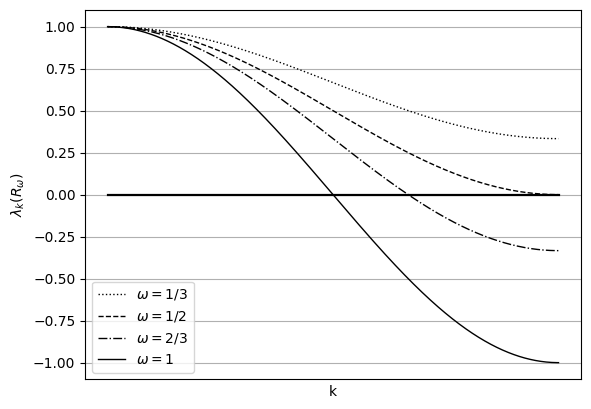
\includegraphics[width=0.45\textwidth]{p6.png}
  \caption{Reproduce Fig. 2.7}
\end{figure}

\begin{lstlisting}[language=python]
  X = np.linspace(0, 6, 1000)
  W = [1/3, 1/2, 2/3, 1]
  Y = []
  for w in W:
      Y.append([1-2*w*m.sin(x*pi/2/6)**2 for x in X])
  plt.plot(X, Y[0], linewidth=1, label="$\omega=$1/3", linestyle=':' , color = 'black')    
  plt.plot(X, Y[1], linewidth=1, label="$\omega=$1/2", linestyle='--', color = 'black')
  plt.plot(X, Y[2], linewidth=1, label="$\omega=$2/3", linestyle='-.', color = 'black')
  plt.plot(X, Y[3], linewidth=1, label="$\omega=$1"  , linestyle='-' , color = 'black')
  plt.grid(True)
  plt.ylabel("$\lambda_k(R_{\omega})$")
  plt.xlabel("k")
  plt.xticks([])
  plt.plot(X, [0]*1000, linewidth=1.6, color='black')
  plt.legend(loc = "lower left")
\end{lstlisting}

\end{solution}

\begin{prob}[Exercise 9.21]
  Write a program to reproduce Figure 2.8
  in the book by Briggs et al. [2000], verifying that regular
  Jacobi is only good for damping modes $16 \le k \le 48$. In
  contrast, for $\omega = \frac23$, 
  the modes $16 \le k < 64$ are all damped out quickly.
\end{prob}

\begin{solution}
如下图所示,不加权 Jacobi 方法的迭代次数在 $16 \le k \le 48$ 时
比较小,在 $k<16,k>48$ 的时候比较大,而加权 Jacobi 迭代(取 $\omega = \frac23$)
在 $16 \le k \le 64$ 的迭代次数都比较小。

\begin{figure}[H]
\centering
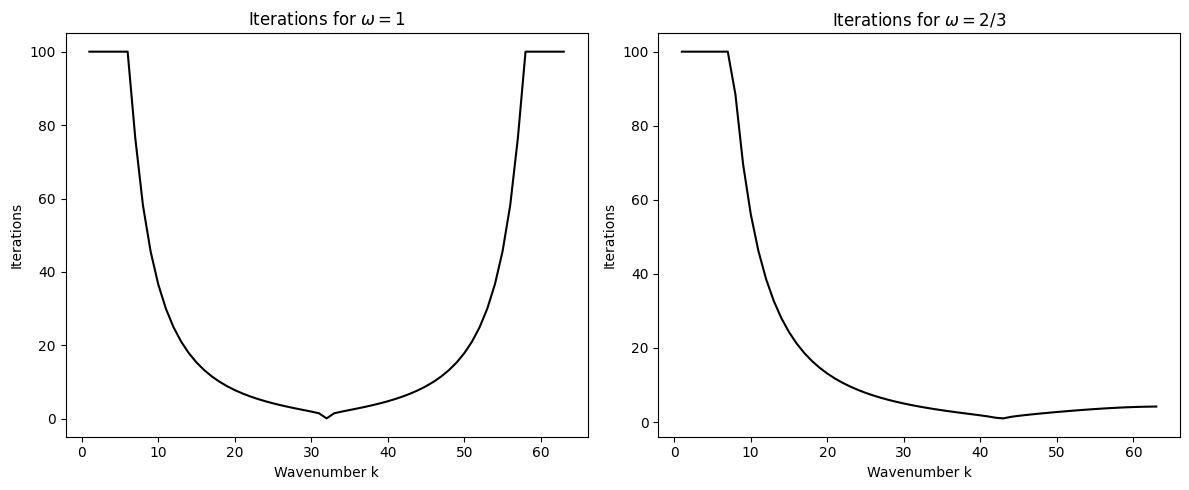
\includegraphics[width=0.9\textwidth]{p7.png}
\end{figure}
\begin{lstlisting}[language=python]
import math as m
n = 64
X = [i for i in range(1, n)]
Y1 = []
Y2 = []
def lambda_k(k, o):
    return 1-2*o*m.sin(k*pi/2/64)**2

def get_n(k, o):
    return min(100, (m.log(0.01) / m.log(abs(lambda_k(k, o)))))

for i in X:
    Y1.append(get_n(i, 1))
    Y2.append(get_n(i, 2/3))

plt.figure(figsize=(12, 5))

plt.subplot(1, 2, 1)
plt.plot(X, Y1, color='black', label='$\omega=1$')
plt.xlabel("Wavenumber k")
plt.ylabel("Iterations")
plt.title('Iterations for $\omega=1$')
plt.subplot(1, 2, 2)
plt.plot(X, Y2, color='black', label='$\omega=2/3$')
plt.xlabel("Wavenumber k")
plt.ylabel("Iterations")
plt.title('Iterations for $\omega=2/3$')
plt.tight_layout()
\end{lstlisting}

\end{solution}

\begin{prob}[Exercise 9.35]
  Show that, for $\nu_1 = \nu_2 = 1$, the computational cost of 
  an FMG cycle is less than $\frac2{(1-2^{-D})^2} \text{WU}$. Give
  upper bounds as tight as possible for computational costs of
  an FMG cycle for $D = 1, 2, 3$.
\end{prob}

\begin{proof}
  在 (FMG-3) 这一步,需要 V-cycles,根据 Lemma 9.33,设最密网格为 $2^m$,宽度为 $h$,
  设当前位于网格 $\Omega^{2^k h}(k = 0, 1, \dots, m)$ 上,
  那么在忽略网格内转移后,计算成本为($\nu_1 = \nu_2 = 1$)
  \[
    2\text{WU} (2^{-kD} + 2^{-(k+1)D} + \cdots + 2^{-mD})
  \]
  考虑在每一个网格上执行 (FMG-3) 这一步的总计算成本,
  \[
    2\text{WU} \sum_{i = 0}^{m} \sum_{j = i}^{m} 2^{-jD} 
   = 2\text{WU} \sum_{i = 0}^m \dfrac{2^{-iD} - 2^{-(m+1)D}}{1 - 2^{-D}}
   < 2\text{WU} \sum_{i = 0}^m \dfrac{2^{-iD}}{1 - 2^{-D}}
   = \dfrac{2}{1 - 2^{-D}}\text{WU} \sum_{i = 0}^m 2^{-iD}
   < \dfrac{2}{(1 - 2^{-D})^2} \text{WU}
  \]

  当 $D = 1, 2, 3$ 时,分别有上界 $8\text{WU}, \dfrac{32}{9} \text{WU}, \dfrac{128}{49}\text{WU}$。
\end{proof}


\begin{prob}[Exercise 9.41]
Rewrite (9.32) as
\[
  TG \begin{bmatrix}\wB_k \\ \wB_{k'}\end{bmatrix} 
  = \begin{bmatrix}
      \lambda_k^{\nu_1 + \nu_2}s_k &
      \lambda_k^{\nu_1}\lambda_{k'}^{\nu_2}s_k \\
      \lambda_{k'}^{\nu_1}\lambda_k^{\nu_2} &
      \lambda_{k'}^{\nu_1 + \nu_2}c_k
    \end{bmatrix} 
    \begin{bmatrix}\wB_k \\ \wB_{k'}\end{bmatrix}
  = \begin{bmatrix}c_1 & c_2 \\ c_3 & c_4\end{bmatrix} 
    \begin{bmatrix}\wB_k \\ \wB_{k'}\end{bmatrix}  
\]
Explain why the magnitude of all four $c_i$’s are small. Deduce
the main conclusion $\rho(TG) \approx 0.1$ by reproducing the
plots in Figure 9.4 of the damping coefficients of two-grid
correction with weighted Jacobi for $n = 64$ and $\omega = \frac23$
. The horizontal axis represents the wavenumber $k$. Repeat the
plots for $n = 128$ to show the independence of $\rho (T G) \approx 0.1$
from the grid size.
\end{prob}

\begin{solution}
因为 $\lambda_k, \lambda_{k'}, s_k, c_k \in [0, 1]$,而 $\nu_1, \nu_2 \in \mathbb{N}^*$,
所以,可以通过增大 $\nu_1, \nu_2$ 让 $c_1, c_2, c_3, c_4$ 变得很小。
\begin{lstlisting}[language=python]
  n = 64
  def lambda_k(k, o=2/3):
      return 1-2*o*m.sin(k*pi/2/n)**2
  def c(k):
      return m.cos(k*pi/2/n)**2
  def s(k):
      return m.sin(k*pi/2/n)**2
  K1 = range(1, (n//2)+2)
  K2 = range((n//2), n+1)
  args = [[0, 0], [0, 2], [1, 1], [2, 0], [2, 2], [4, 0]]
  plt.figure(figsize=(15, 10))
  
  def rho(matrix):
      eigenvalues, _ = np.linalg.eig(matrix)
      max_eigenvalue_abs = np.max(np.abs(eigenvalues))
      return max_eigenvalue_abs
  
  for i, [nu1, nu2] in enumerate(args, start=1):
      plt.subplot(2, 3, i)
      C1 = []
      C2 = []
      C3 = []
      C4 = []
      R = []
      for k in K1:
          k_ = n - k
          C1.append(lambda_k(k)**(nu1+nu2)*s(k))
          C3.append(lambda_k(k_)**nu1*lambda_k(k)**nu2*c(k))
      for k in K2:
          k_ = n - k
          C2.append(lambda_k(k_)**nu1*lambda_k(k)**nu2*s(k_))
          C4.append(lambda_k(k)**(nu1+nu2)*c(k_))
      id1 = 0
      id2 = len(C2) - 1
      for k in K1:
          k_ = n - k
          c1 = C1[id1]
          c2 = C2[id2]
          c3 = C3[id1]
          c4 = C4[id2]
          id1 = id1 + 1
          id2 = id2 - 1
          R.append(rho([[c1, c2], [c3, c4]]))
      plt.plot(K1, R,  color = 'red', label = 'rho')
      plt.plot(K1, C1, color = 'black', linestyle = '-', linewidth = 1, label = 'c1')
      plt.plot(K2, C2, color = 'black', linestyle = '-.', linewidth = 1, label = 'c2')
      plt.plot(K1, C3, color = 'black', linestyle = ':', linewidth = 1, label = 'c3')
      plt.plot(K2, C4, color = 'black', linestyle = '-', linewidth = 2, label = 'c4')
      plt.title("$v_1 = {}, v_2 = {}$".format(nu1, nu2))
      plt.legend()
\end{lstlisting}

在上述代码中,还计算了相应的 $\rho(A)$ 的值, 
通过比较 $n = 64, n= 128$ 的图像可以发现 $\rho(A) \approx 0.1$ 且与网格大小没有关系。

\begin{figure}[H]
  \centering
  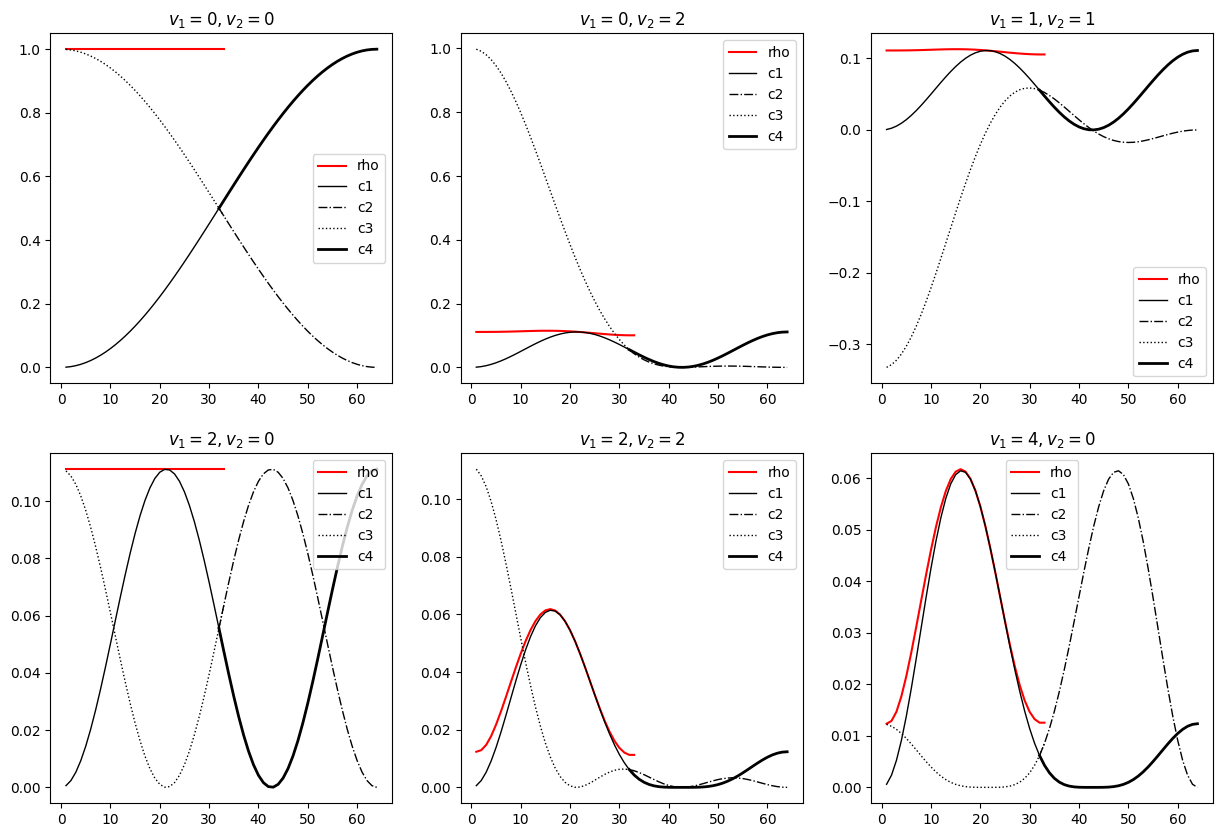
\includegraphics[width=0.9\textwidth]{p8.png}
  \caption{Reproduce of figures of $n = 64$}
\end{figure}
\begin{figure}[H]
  \centering
  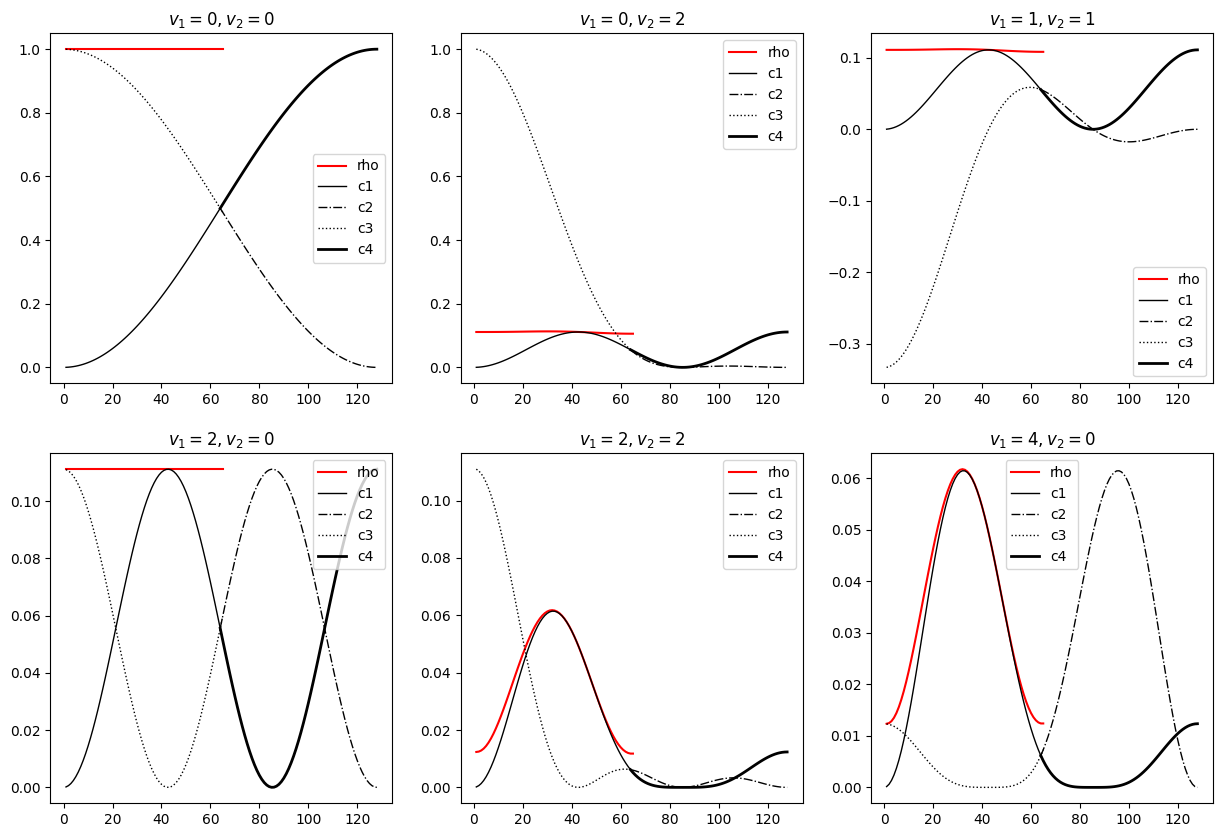
\includegraphics[width=0.9\textwidth]{p9.png}
  \caption{Reproduce of figures of $n = 128$}
\end{figure}
\end{solution}

\begin{prob}[Exercise 9.45]
\textbf{Lemma 9.44.}\quad The full-weighting operator satisfies
\[
  \dim \mathcal{R}(I_h^{2h}) = \frac{n}2 - 1,\quad
  \dim \mathcal{N}(I_h^{2h}) = \frac{n}2.
\]
\end{prob}

\begin{proof}
  全加权算子 $I_h^{2h}$ 为
  \[
    I_h^{2h} = \frac14 \begin{bmatrix}
      1 & 2 & 1 & & & & & \\
      & & 1 & 2 & 1 & & & \\
      & & & & \ddots & \ddots & \ddots & \\
      & & & & & 1 & 2 & 1
    \end{bmatrix}
  \]
  所以 $I_h^{2h}$ 满秩,
  \[
    \dim \mathcal{R}(I_h^{2h}) = \text{rank} (I_h^{2h}) = \frac{n}2 - 1
  \]
  根据线性映射基本定理,
  \[
    n - 1 = \dim \RBB^{n-1} = \dim \mathcal{R}(I_h^{2h}) + \dim \mathcal{N}(I_h^{2h}).
  \]
  所以,$\dim \mathcal{N}(I_h^{2h}) = 
  (n - 1) - \mathcal{R}(I_h^{2h}) 
  = (n - 1) - \left(\frac{n}2 - 1\right) 
  = \frac{n}2$
\end{proof}

\nocite{*}
\printbibliography[heading=bibintoc, title=\ebibname]

\end{document}